\section{Auswertung}
\subsection{Bestimmung der RC-Konstanten durch die Entladungskurve}
In der Abbildung %\ref{fig:kurve}
ist die zur Ausmessung verwendete Entladungskurve des Kondensators, welcher
durch einen Generator mit der der Frequenz von $\nu$ = 50 $\si{\hertz}$ mit
 U =12.00 $\si{\volt}$ aufgeladen wurde, zu sehen.
\begin{figure}[H]
  \centering
  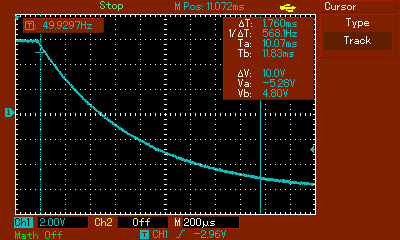
\includegraphics{kurve}
  \caption{Entladungskurve}
  \label{fig:kurve}
\end{figure}
\noindent In Tabelle \ref{tab:tabe1} sind die aus ihr gewonnenen Messwertpaare zusammen mit
dem Verhältniss $ \frac{U}{U_0} $ und dessen Logarithmus, welcher zur
Auswertung nötig ist, abzulesen.
\begin{table}[H]
  \centering
  \caption{Messwerte zur Bestimmung der RC-Konstanten}
  \label{tab:tabe1}
    \begin{tabular}{c c c c}
    \toprule
    $ t \: / \si{\milli\second} $ & $ U_C \: / \si {\volt} $ & $\frac{U_C}{U_0} $
    & $ \ln{\frac{U_C}{U_0}} $ \\
    \midrule
    0.000 & 12.00 & 1.000 & 0.000 \\
    0.080 & 10.88 & 0.907 & -0.098 \\
    0.160 & 9.84 & 0.820 & -0.198 \\
    0.240 & 8.96 & 0.747 & -0.292 \\
    0.320 & 8.16 & 0.680 & -0.386 \\
    0.400 & 7.44 & 0.620 & -0.478 \\
    0.480 & 6.80 & 0.567 & -0.568 \\
    0.560 & 6.16 & 0.513 & -0.667 \\
    0.640 & 5.68 & 0.473 & -0.748 \\
    0.720 & 5.20 & 0.433 & -0.836 \\
    0.800 & 4.72 & 0.393 & -0.933 \\
    0.880 & 4.32 & 0.360 & -1.022 \\
    0.960 & 4.00 & 0.333 & -1.099 \\
    1.040 & 3.68 & 0.307 & -1.182 \\
    1.120 & 3.36 & 0.280 & -1.273 \\
    1.200 & 3.12 & 0.260 & -1.347 \\
    1.280 & 2.88 & 0.240 & -1.427 \\
    1.360 & 2.64 & 0.220 & -1.514 \\
    1.440 & 2.48 & 0.207 & -1.577 \\
    1.520 & 2.32 & 0.193 & -1.643 \\
    1.600 & 2.16 & 0.180 & -1.715 \\
    1.680 & 2.00 & 0.167 & -1.792 \\
    1.760 & 2.00 & 0.167 & -1.792 \\

      \bottomrule
    \end{tabular}
\end{table}

\noindent Zur Bestimmung der RC-Konstante wird dann der Logarithmus des Verhältnisses gegen
die Zeit in einem halblogarithmischen Diagramm aufgetragen, wie in Abbildung
\ref{fig:gerade} zu sehen ist, und eine lineare Ausgleichsrechnung durchgeführt.
\begin{figure}[H]
  \centering
  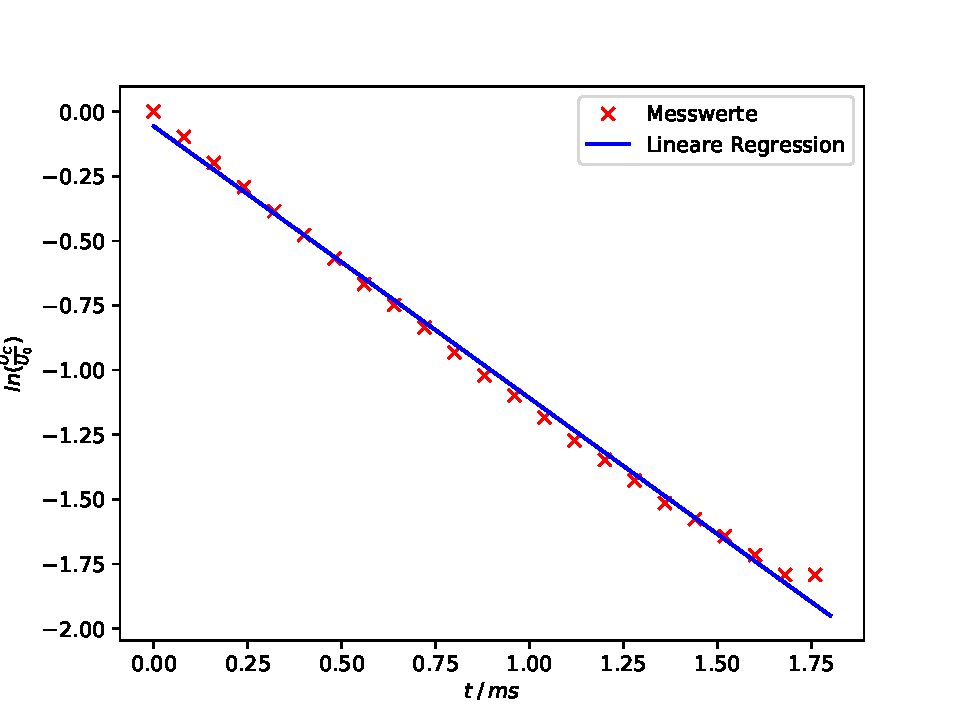
\includegraphics{plot1.pdf}
  \caption{Halblogaritmisches Diagramm des Entladevorgangs}
  \label{fig:gerade}
\end{figure}
\noindent Hieraus ergeben sich für die Steigung a und den y-Achsenabschnitt die Parameter
\begin{align*}
  a&= \SI{-1.0513(15)}{1\per\milli\second} \\
  b&= -0.057 \pm 0.016
\end{align*}
Nach Umstellen der Gleichung \ref{eqn:entladung} ergibt sich für die RC Konstante:
\begin{equation}
  \text{RC} = -\frac{t}{\log\left({\frac{U}{U_0}}\right)} = -\frac{1}{a} =
  \SI{0.951(14)}{\milli\second}
\end{equation}
\subsection{Bestimmung der RC-Konstanten durch Anregung mit einer Sinusspannung}
Eine weiter Methode zur Bestimmung der RC-Konstanten ist das Anlegen einer
Sinusspannung, wobei die Frequenz $ \nu $ variiert wird und die entsprechenden
Amplituden gemessen, wie in Tabelle \ref{tab:tabe2} zu sehen ist.
\begin{table}[H]
  \centering
  \caption{Amplitude in Abhängigkeit der Frequenz}
  \label{tab:tabe2}
    \begin{tabular}{c c}
    \toprule
    $ \nu \: / \si{\hertz} $ & $ U_C \: / \si {\volt} $ \\
    \midrule
    10 & 14.85 \\
    30 & 14.65 \\
    70 & 13.94 \\
    100 & 13.15 \\
    300 & 8.40 \\
    700 & 4.28 \\
    1000 & 3.09 \\
    2000 & 1.50 \\
    3000 & 1.01 \\
    4000 & 0.76 \\
    5000 & 0.62 \\

    \bottomrule
    \end{tabular}
\end{table}

\noindent Mit der normierten Spannung wird dann eine Ausgleichsrechnung mit der Funktion
\begin{equation}
  f(x)= \frac{1}{\sqrt{1+a\cdot x^2}}
\end{equation}
durchgeführt, wie in dem halblogarithmischen Diagramm \ref{fig:Ampl} zu sehen ist.
\begin{figure}[H]
  \centering
  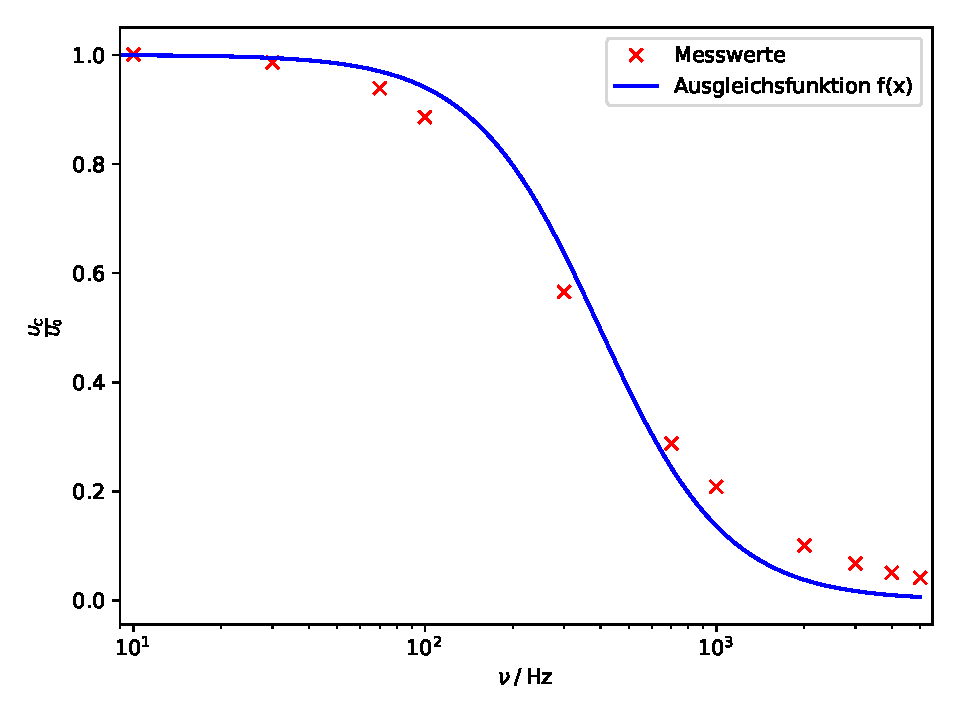
\includegraphics{plot2.pdf}
  \caption{Frequenzabhängigkeit der Amplitude}
  \label{fig:Ampl}
\end{figure}
\noindent Für den Parameter a ergibt sich daraus:
\begin{equation*}
  a= \SI{6.34(98)e-6}{1\per\second}
\end{equation*}
Aus der Gleichung \ref{eqn:amplitude} ergibt sich für die RC-Konstante
somit:
\begin{equation}
  RC = \sqrt{a} =\SI{2.52(20)}{\milli\second}
\end{equation}
\subsection{Bestimmung der RC-Konstanten durch die Phasenverschiebung}
Im dritten Versuchsteil wird die Phasenverschiebung zwischen der Spannung
des Generators und des RC-Glieds verwendet um die RC-Konstante zu bestimmen. Dazu
werden die zeitliche Verschiebung $a$ und die Schwingungslänge $b$ gemessen,
woraus sich mit
\begin{equation}
  \phi = \frac{a}{b} \cdot 2\pi
\end{equation}
die Phasenverschiebung berechnen lässt, wie in Tabelle \ref{tab:tabe3}
dargestellt ist.
\begin{table}[H]
  \centering
  \caption{Phasenverschiebung in Abhängigkeit der Frequenz}
  \label{tab:tabe3}
    \begin{tabular}{c c c c}
    \toprule
    $ \nu \: / \si{\hertz} $ & $ a \: / \si {\milli \second} $ & $ b \:
     / \: \si{\milli \second} $
    & $ \phi \: / \: rad $ \\
    \midrule
    10 & 0.40 & 100.00 & 0.025 \\
    30 & 0.80 & 33.33 & 0.151 \\
    70 & 0.80 & 14.29 & 0.352 \\
    100 & 0.88 & 10.00 & 0.553\\
    300 & 0.48 & 3.33 & 0.906\\
    700 & 0.28 & 1.43 & 1.230\\
    1000 & 0.22 & 1.00 & 1.382\\
    2000 & 0.11 & 0.50 & 1.382\\
    3000 & 0.08 & 0.33 & 1.523\\
    4000 & 0.06 & 0.25 & 1.508\\
    5000 & 0.05 & 0.20 & 1.571\\

      \bottomrule
    \end{tabular}
\end{table}

\noindent Anschließend wird wieder eine Ausgleichsrechnung durchgeführt, diesmal mit der
Funktion
\begin{equation}
  f(x) = arctan (c \cdot x)
\end{equation}
Hieraus ergibt sich für den Parameter c
\begin{equation*}
  c = \SI{4.85(33)e-3}{\second}
\end{equation*}
Aus Gleichung \ref{eqn:phi} folgt somit
\begin{equation}
   RC = c = \SI{4.85(33)}{\milli\second}
\end{equation}
Die Ausgleichsfunktion ist zusammen mit den Wertepaaren in dem halblogarithmischen
Diagramm \ref{fig:phase} dargestellt.
\begin{figure}[H]
  \centering
  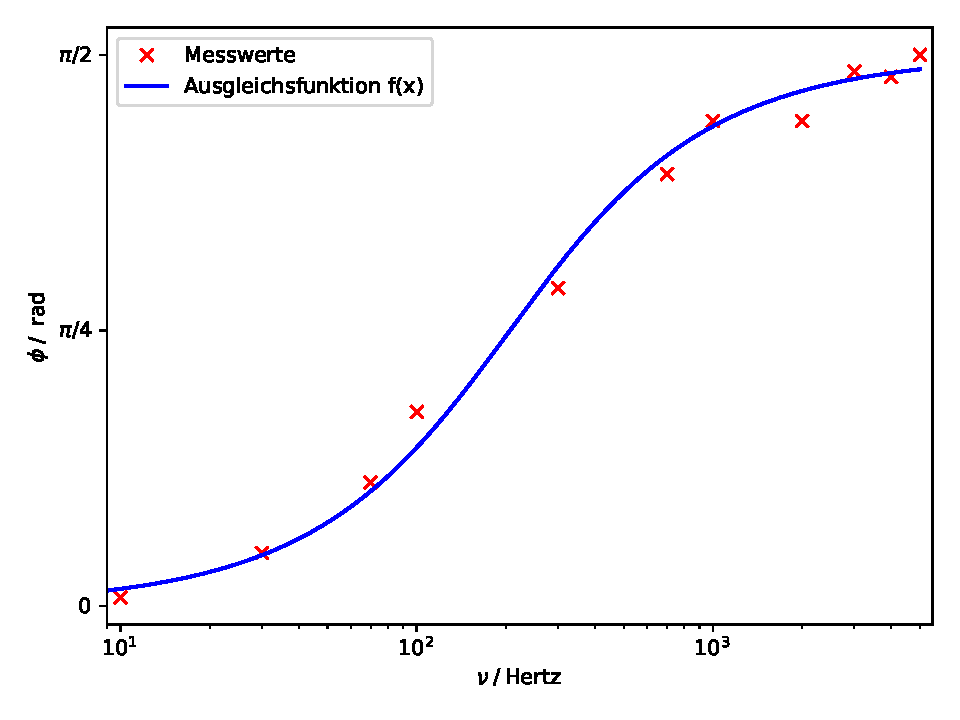
\includegraphics{plot3.pdf}
  \caption{Frequenzabhängigkeit der Phasenverschiebung}
  \label{fig:phase}
\end{figure}

\noindent Mit den nun bereits vorhandenen Messwerten aus den Tabellen \ref{tab:tabe2}
und \ref{tab:tabe3} lässt sich nun ein Polar-Plot erstellen(Abbildung \ref{fig:polar}),
in welchem die Messwerte zusammen mit der Theoriekurve dargestellt werden.
\begin{figure}[H]
  \centering
  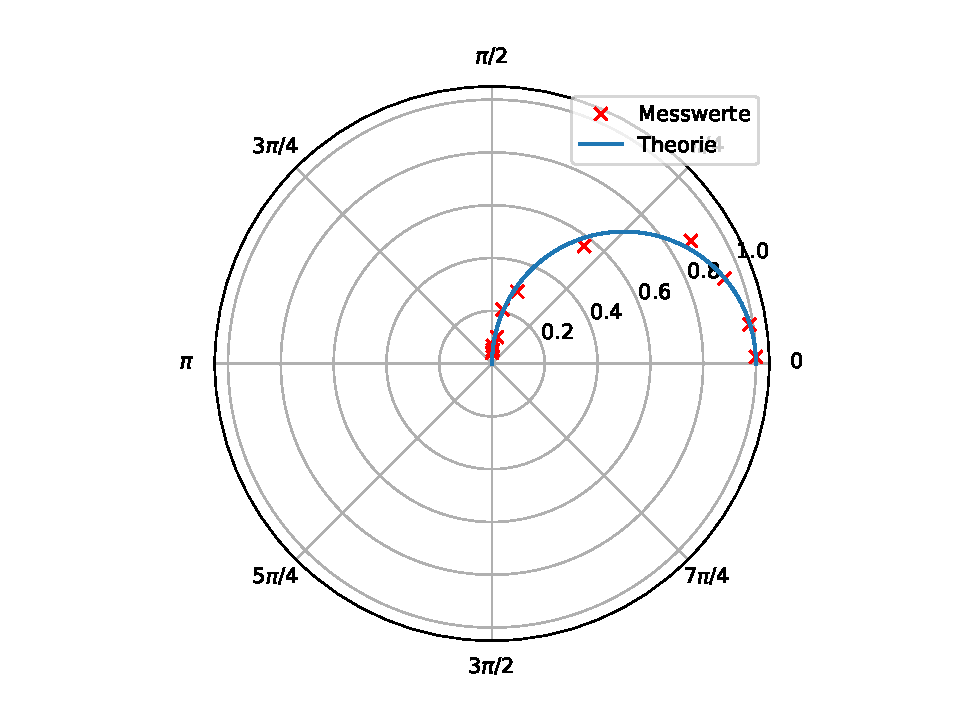
\includegraphics{plot4.pdf}
  \caption{Polare Darstellung der Amplitude und Phasenverschiebung}
  \label{fig:polar}
\end{figure}

\subsection{Der RC-Kreis als Integrator}
Schlussendlich soll noch gezeigt werden, dass der RC-Kreis als Integrator
fungieren kann, was durch die folgenden Grafiken deutlich wird. Dabei ist die
Generatorfrequenz in gelb und die resultierende Frequenz des RC-Kreises in blau
dargestellt. Zu beachten ist, dass hierbei unterschiedliche Skalierungen
vorgenommen wurden.

\subsubsection{Sinusschwingen}
Eine Sinusspannung der Form
\begin{equation*}
  f(x) = a\cdot \sin{x}
\end{equation*}
ergibt durch Integration die Stammfunktion
\begin{equation*}
  F(x) = -a\cdot \cos{x} + C
\end{equation*}
\begin{figure}[H]
  \centering
  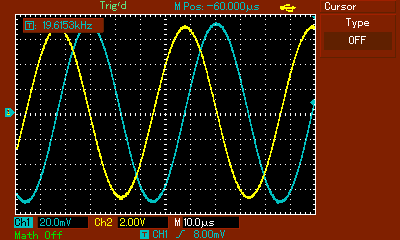
\includegraphics{sinus.png}
  \caption{Integration der Sinusspannung}
  \label{fig:sinus}
\end{figure}
\subsubsection{Dreieckspannung}
Eine Dreieckspannung der Form
\begin{equation*}
  f(x) = \begin{cases}
         b \cdot x  , & -a < x < a \\
         -b \cdot x  , & a < x < 3a
       \end{cases}
\end{equation*}
ergibt durch Integration die Stammfunktion
\begin{equation*}
  F(x) = \begin{cases}
         \frac{b}{2} \cdot x^2  , & -a < x < a \\
         -\frac{b}{2} \cdot x^2  , & a < x < 3a
       \end{cases}
\end{equation*}
\begin{figure}[H]
  \centering
  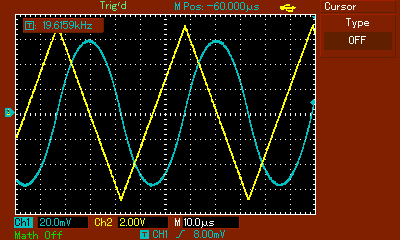
\includegraphics{Dreieck.png}
  \caption{Integration der Dreieckspannung}
  \label{fig:dreieck}
\end{figure}
\subsubsection{Rechteckspannung}
Eine Rechteckspannung der Form
\begin{equation*}
  f(x) = \begin{cases}
         b , & 0 < x < a \\
         -b , & a < x < 2a
       \end{cases}
\end{equation*}
ergibt durch Integration die Stammfunktion
\begin{equation*}
  f(x) = \begin{cases}
         b \cdot x , & 0 < x < a \\
         -b \cdot x, & a < x < 2a
       \end{cases}
\end{equation*}
\begin{figure}[H]
  \centering
  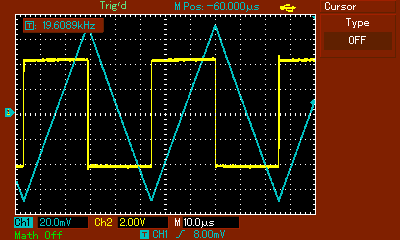
\includegraphics{rechteck.png}
  \caption{Integration der Rechteckspannung}
  \label{fig:rechteck}
\end{figure}
